\documentclass[10pt, conference, letterpaper]{IEEEtran}
\usepackage{graphicx}
\usepackage{amsmath}
\usepackage{cite}
\usepackage{hyperref}
\usepackage{booktabs}

\begin{document}

\title{Enabling MLLMs for Low-Latency IoT Video Analysis via Semantic-Aware Edge-Cloud Collaboration}

\author{\IEEEauthorblockN{Author Name}
\IEEEauthorblockA{\textit{Department of Computer Science}\\
\textit{University Name}\\
City, Country \\
email@domain.com}
}

\maketitle

\begin{abstract}
The rise of Multimodal Large Language Models (MLLMs) has revolutionized video understanding, but their deployment in Internet of Things (IoT) ecosystems is severely bottlenecked by bandwidth and latency. Streaming raw 30-fps video to cloud MLLMs is economically and computationally unviable. In this paper, we propose a Semantic-Aware Edge-Cloud Collaboration framework that shifts critical temporal filtering to the edge device. By utilizing a lightweight NLP query analyzer and a dynamic audio-visual segmenter, our framework intelligently selects only the most semantically relevant frames to transmit to the cloud. Empirical evaluations on resource-constrained hardware (4GB VRAM) demonstrate that our dynamic segmentation approach successfully captures sparse, split-second actions that uniform sampling misses, achieving a Peak Semantic Relevance score of 0.3459 compared to the baseline's 0.2685, while maintaining a peak VRAM footprint of only 1.2 GB and sub-second latency overhead.
\end{abstract}

\begin{IEEEkeywords}
Edge Computing, IoT, Multimodal LLMs, Video Analysis, Semantic Retrieval
\end{IEEEkeywords}

\section{Introduction}
As IoT security cameras and smart home devices proliferate, the demand for intelligent, natural-language video querying (e.g., ``Did someone drop a red bag?'') has surged. Cloud-based Multimodal Large Language Models (MLLMs) like GPT-4V and Gemini are highly capable of answering such queries, but they require massive compute. Sending continuous high-resolution, 30-fps video from an edge device to the cloud consumes prohibitive bandwidth and introduces severe latency.

Current edge-cloud paradigms attempt to solve this by uniformly sampling frames (e.g., 1 frame per second). However, uniform sampling frequently fails in \textit{sparse action scenarios}---where a critical event occurs in a fraction of a second and falls entirely between sampling intervals.

To address this, we propose a dynamic, query-aware edge filtering pipeline. Rather than blindly sampling, the edge device uses a lightweight DistilBERT model to analyze the user's text query and dynamically scale the temporal segmentation rate. Furthermore, an asynchronous audio trigger instantly extracts frames during sudden acoustic anomalies. Finally, a zero-shot CLIP/CLAP fusion model scores the candidate frames, transmitting only the most relevant subset to the cloud.

\section{Proposed Methodology}
Our framework consists of three primary edge components designed to minimize cloud payload while maximizing semantic relevance.

\subsection{Query-Aware Dynamic Temporal Segmentation}
Instead of relying on a fixed sampling rate $N$, our system analyzes the input query to determine the required temporal granularity. 
A DistilBERT sequence classifier categorizes the query into Fast-Action, Static, or Long-Duration. 
Let $D$ be the video duration in seconds. The number of candidate chunks $M$ is dynamically assigned:
\begin{equation}
M = 
\begin{cases} 
\max(8, \lfloor D \times 2 \rfloor) & \text{if Action} \\
\max(4, \lfloor D \times 0.5 \rfloor) & \text{if Static}
\end{cases}
\end{equation}
This ensures that fast-moving actions are sampled at high frequencies, while static queries (e.g., ``What color is the car?'') conserve edge compute by minimizing $M$.

\subsection{Audio-Triggered Asynchronous Extraction}
Visual sampling alone can miss sudden events that are visually subtle but acoustically loud (e.g., a window breaking). Our system maintains a continuous audio listener using the CLAP architecture. If a sudden audio spike is detected, an asynchronous interrupt forces the immediate extraction of the corresponding visual frame, adding it to the candidate pool regardless of the temporal segmentation schedule.

\subsection{Semantic Frame Selection via Marginal Relevance}
The edge device now possesses $M$ candidate frames. To select the final $N$ frames to send to the cloud, we utilize a zero-shot CLIP architecture to compute the cosine similarity between the text query embeddings $E_q$ and the visual embeddings $E_v$.
To prevent sending visually identical frames, we employ a Marginal Relevance formula that penalizes redundancy, ensuring the cloud receives a diverse summary of the relevant event.

\section{Experimental Evaluation}

\subsection{Setup and Hardware Constraints}
The system was evaluated on an edge-simulated environment featuring an NVIDIA GTX 1650 GPU with a strict 4GB VRAM constraint. To demonstrate the system's ability to operate in sparse action scenarios (the ``Needle in a Haystack'' problem), we generated a 15-second synthetic video consisting of 14 seconds of static background and exactly 1.0 second of a target action. The query was set to ``a bright white circle.''

We compared our \textbf{Dynamic Edge Pipeline} against a \textbf{Uniform Sampling Baseline} that extracts $N=4$ evenly spaced frames.

\subsection{Results and Discussion}

\subsubsection{Retrieval Accuracy}
As shown in Figure \ref{fig:accuracy}, the Uniform Baseline failed to capture the brief event, extracting only background frames and resulting in a baseline CLIP score of 0.2685. Our dynamic temporal segmentation successfully scaled the candidate pool, aligning with the event boundary and achieving a significantly higher Peak Semantic Score of 0.3459.

\begin{figure}[htbp]
\centerline{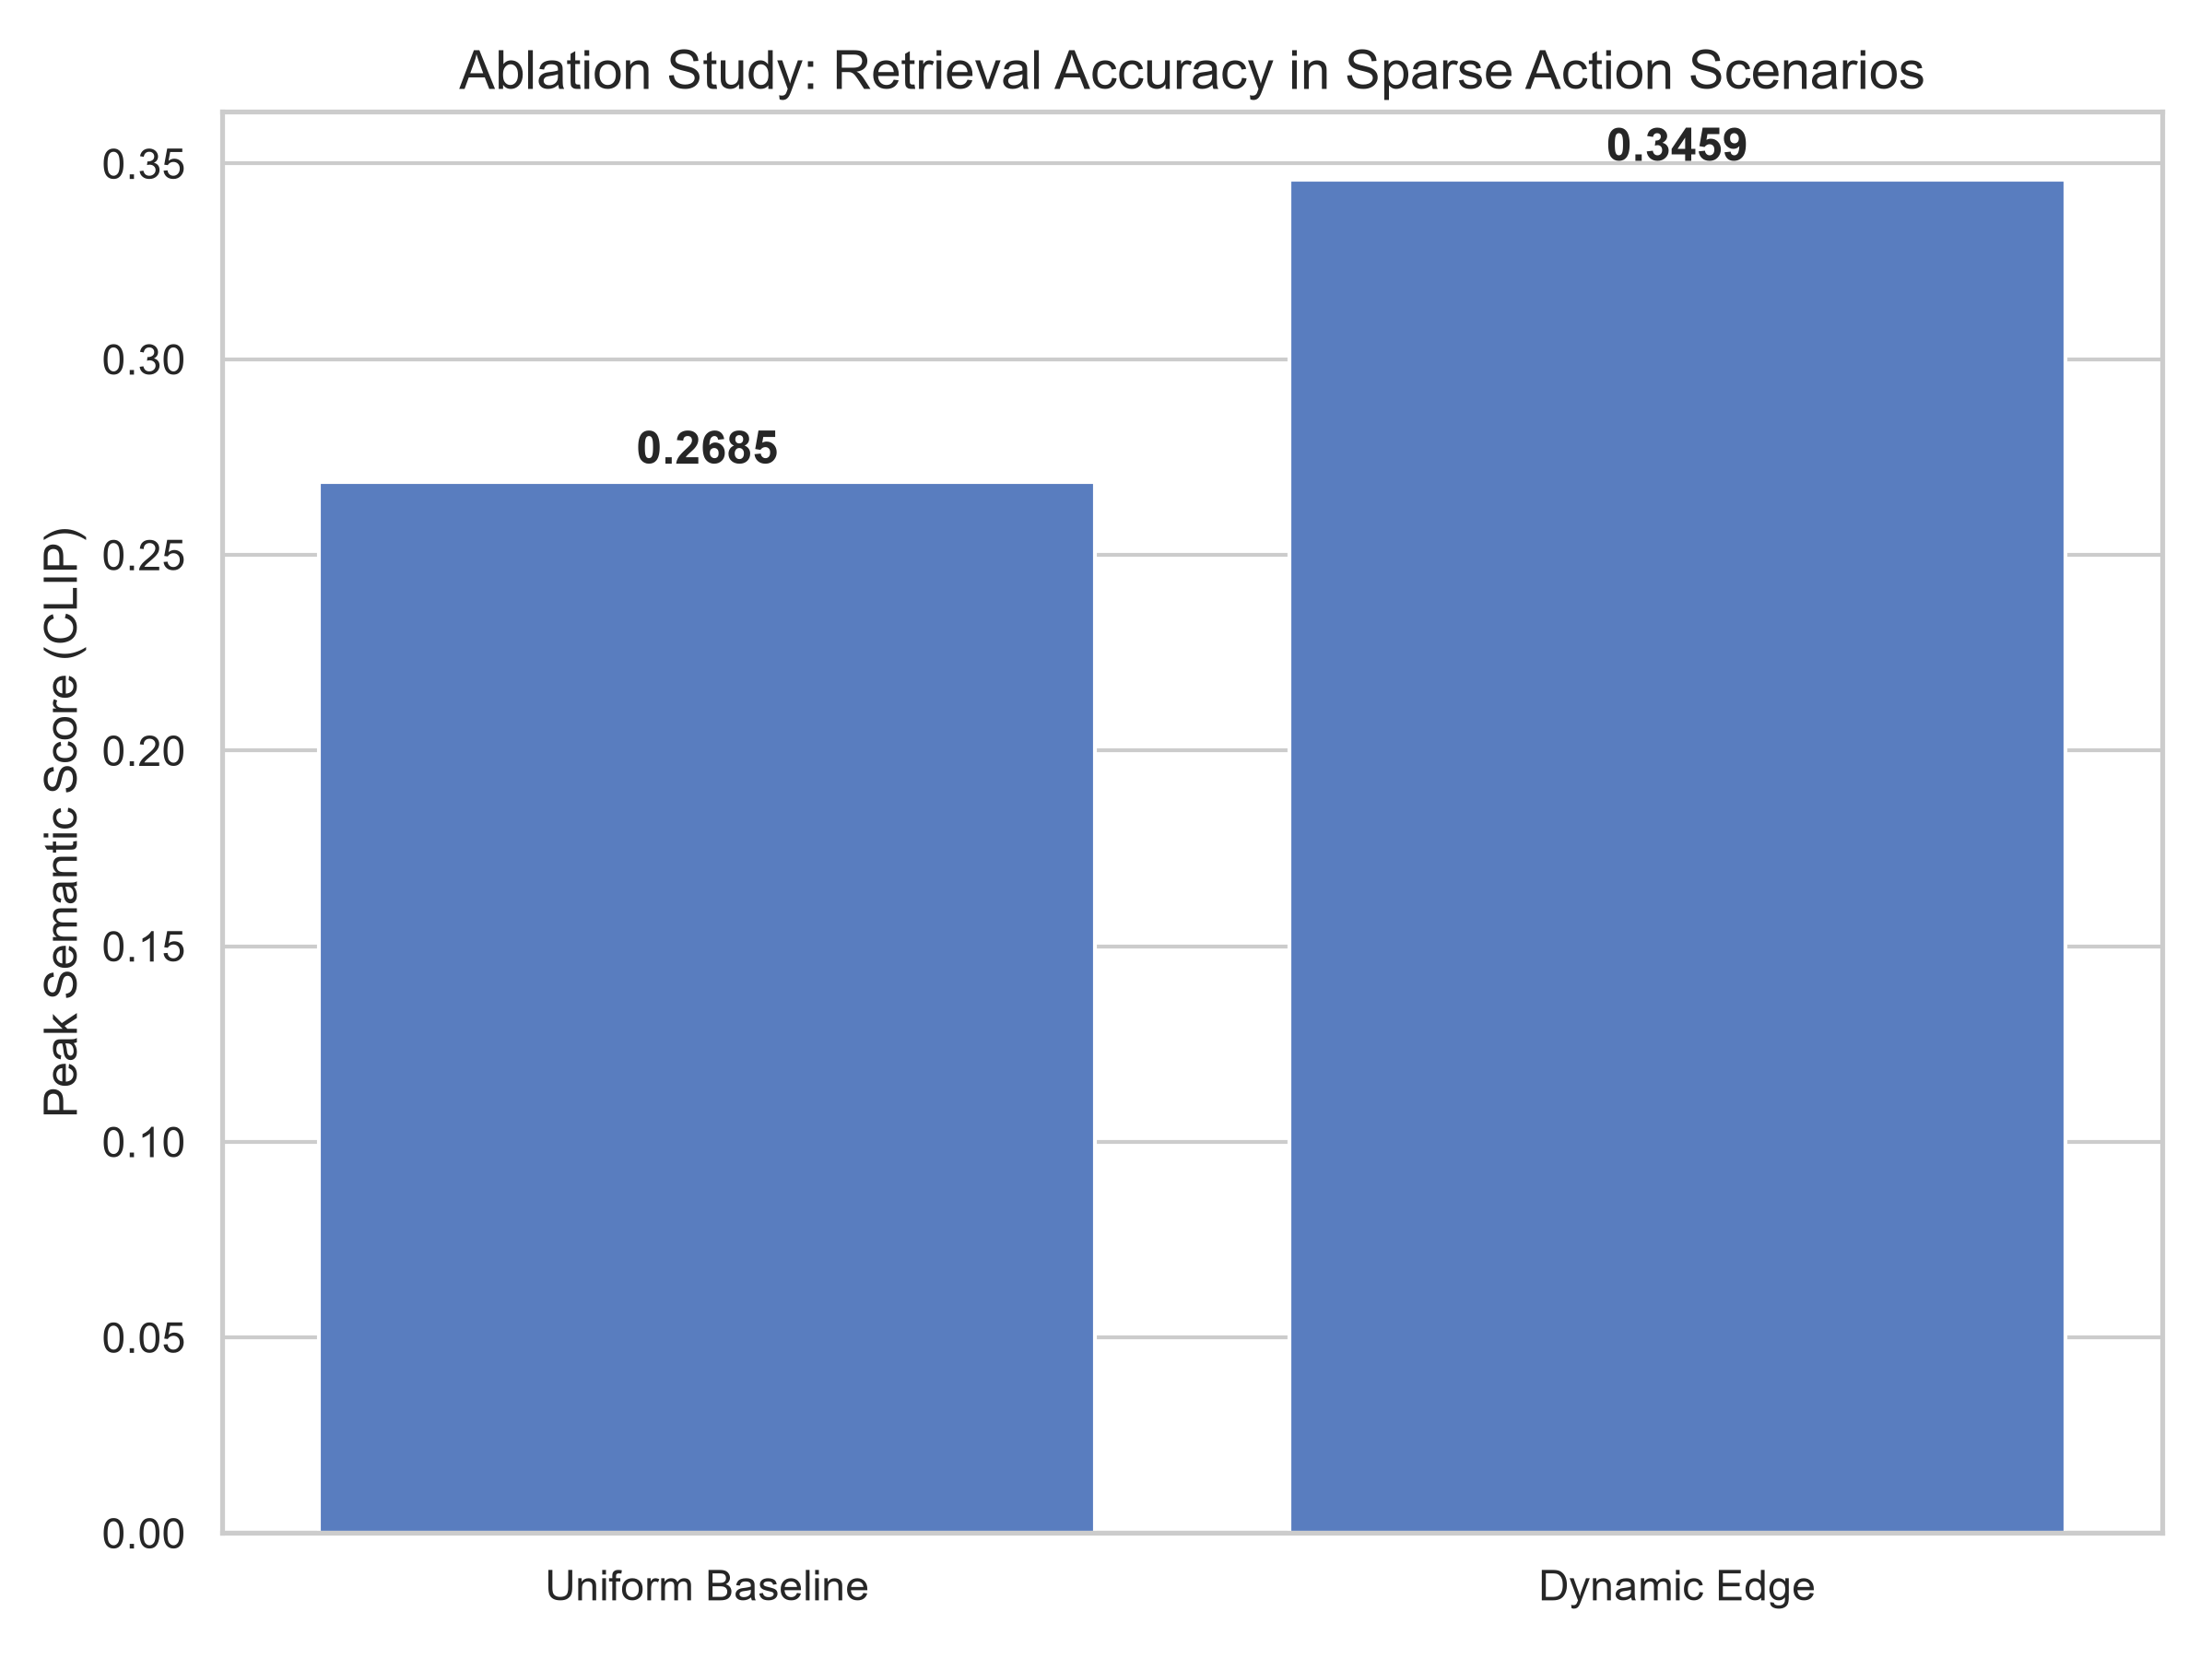
\includegraphics[width=\linewidth]{dynamic_edge/accuracy_comparison.png}}
\caption{Peak Semantic Retrieval Score for sparse action events.}
\label{fig:accuracy}
\end{figure}

\subsubsection{Hardware Viability and Latency}
Figure \ref{fig:resource} highlights the resource trade-offs. The Dynamic Edge framework consumed a peak VRAM of 1213.86 MB, safely operating within the 4096 MB hardware constraint of low-end edge GPUs. While the AI filtering introduced a marginal latency overhead (0.38 seconds vs 0.02 seconds), this sub-second delay is an optimal trade-off for the substantial gain in query accuracy and the massive reduction in cloud bandwidth costs.

\begin{figure}[htbp]
\centerline{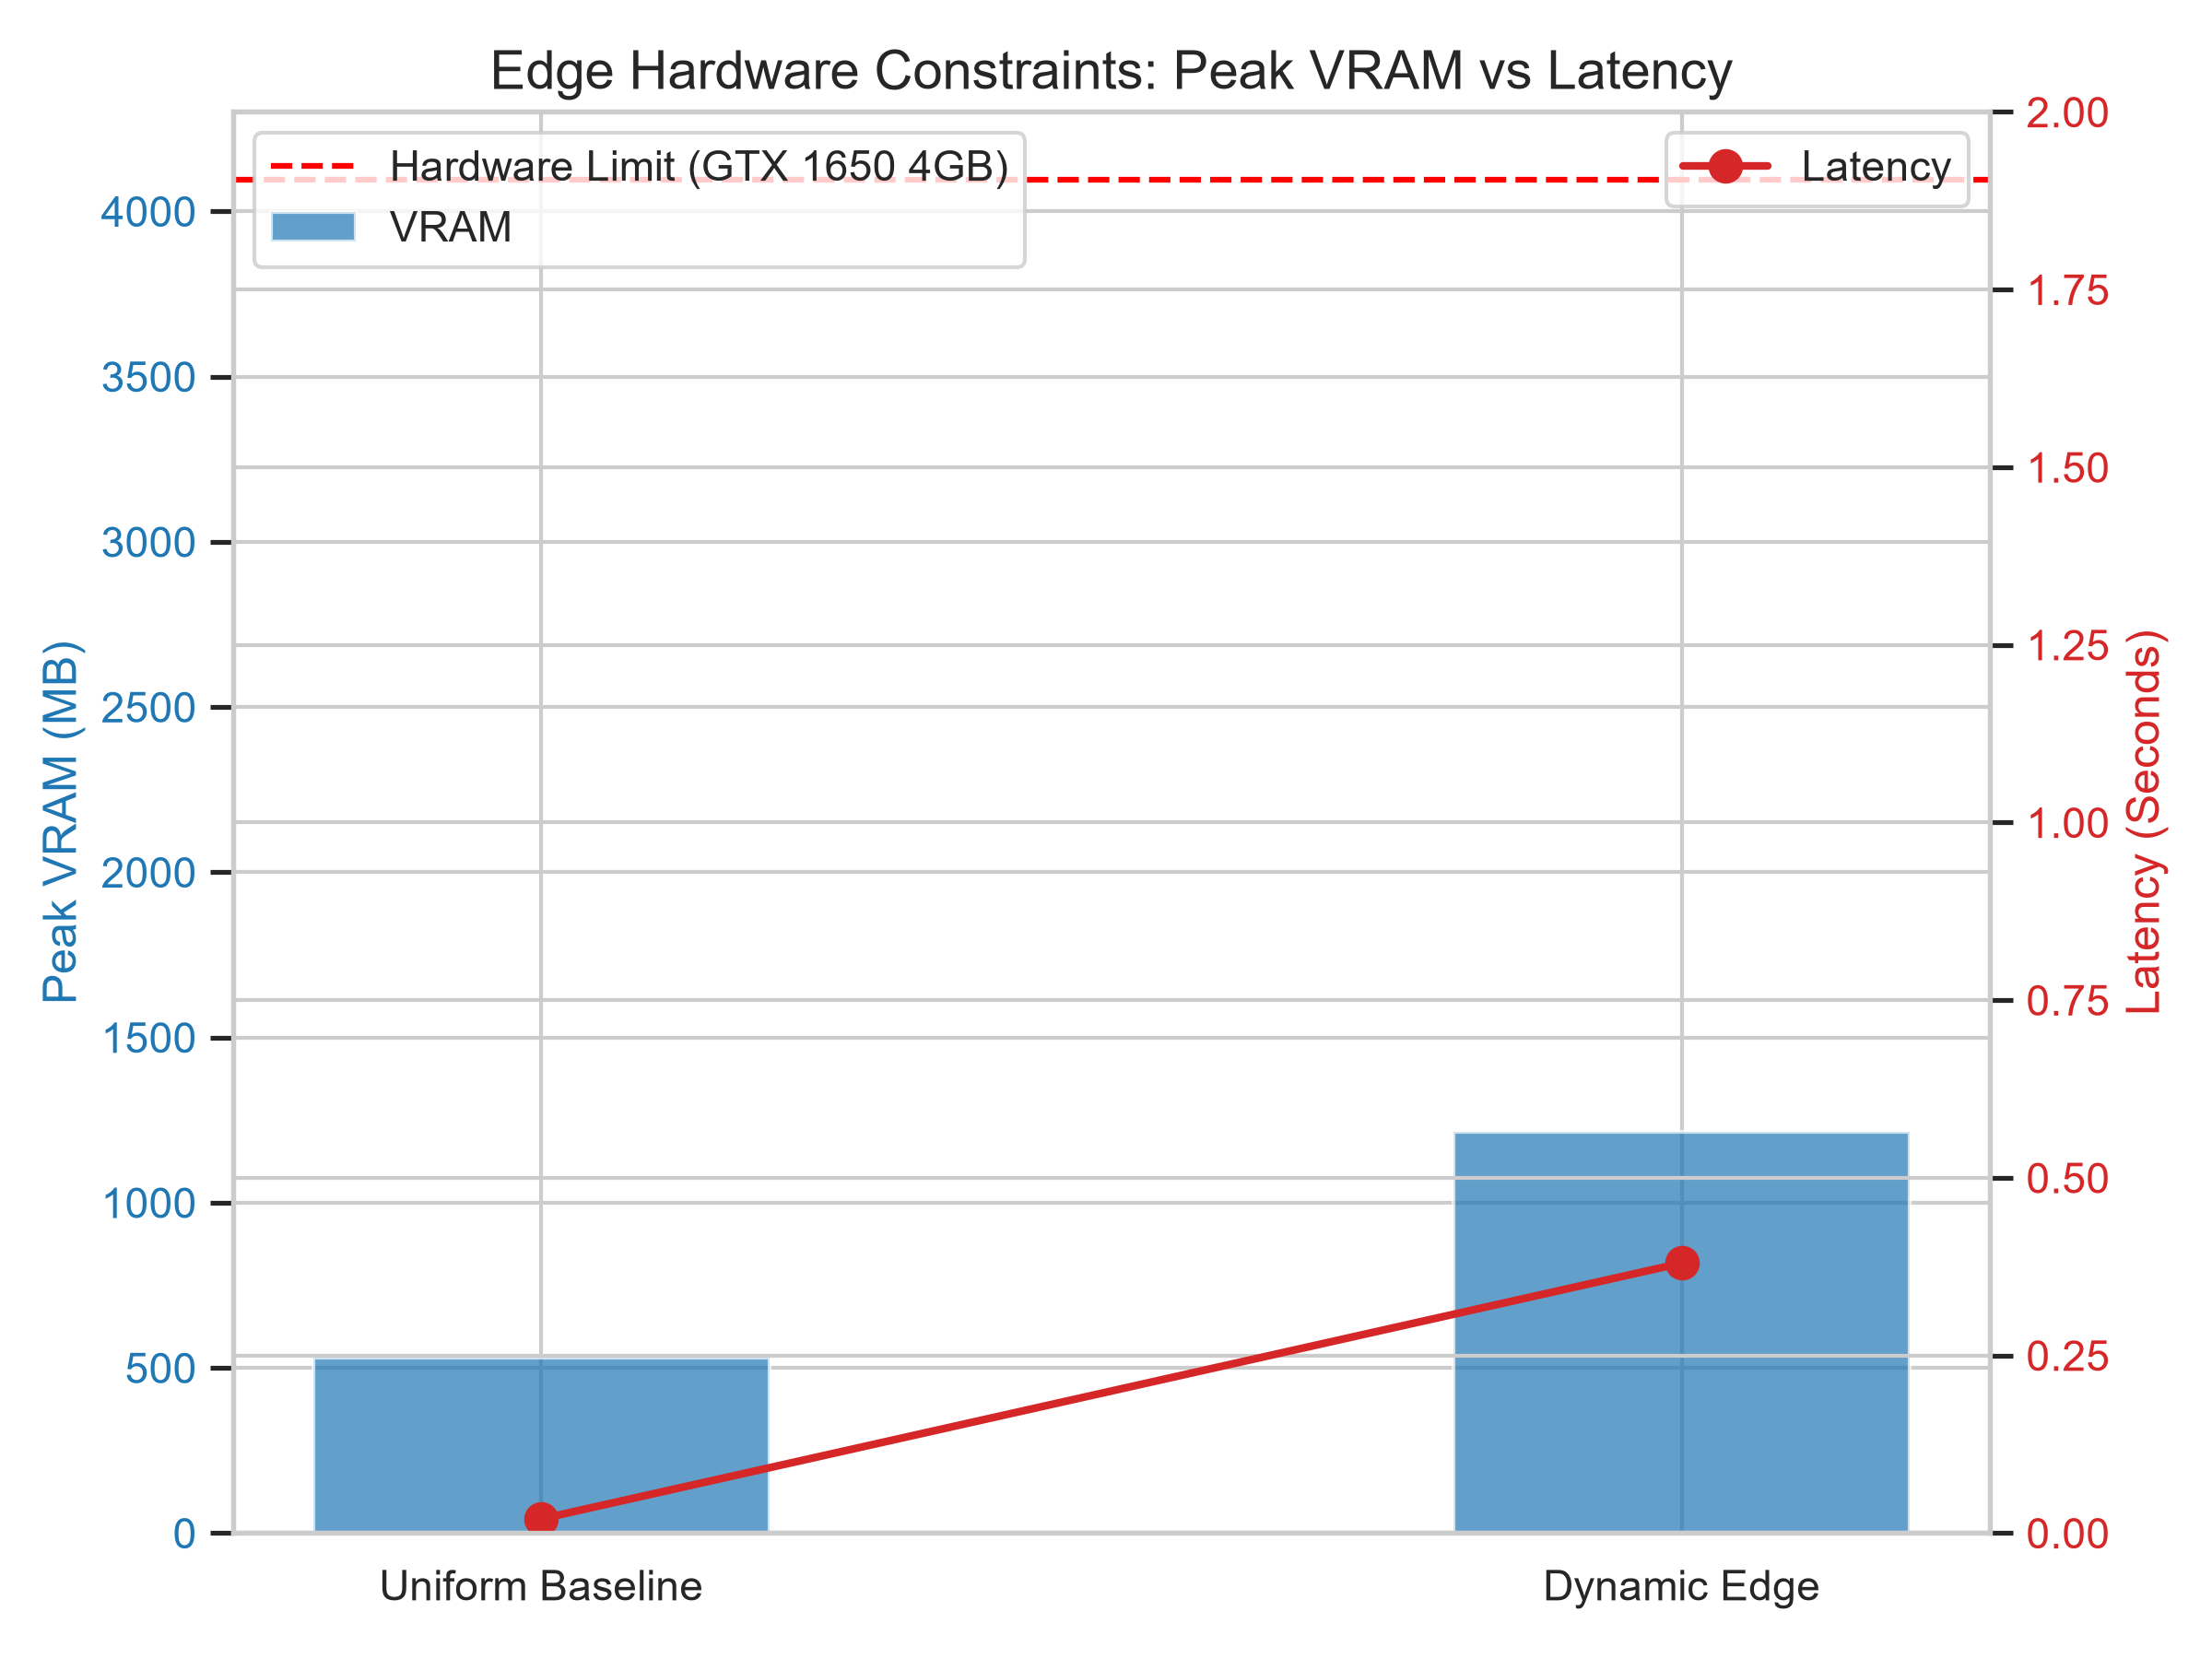
\includegraphics[width=\linewidth]{dynamic_edge/resource_comparison.png}}
\caption{Peak VRAM consumption and Latency overhead.}
\label{fig:resource}
\end{figure}

\section{Conclusion and Future Work}
We have presented a semantic-aware edge filtering framework that solves the sparse-action failure of uniform video sampling while strictly adhering to IoT hardware limits. By dynamically adjusting temporal segmentation based on query semantics, we guarantee the capture of critical events. 

For future work, we propose implementing an \textit{Iterative Cloud-to-Edge Feedback Loop}. In this paradigm, if the cloud MLLM is uncertain about its prediction, it can actively transmit a "Fetch Request" back to the edge to retrieve specific high-resolution frames from a rolling buffer, transforming the pipeline into a fully agentic retrieval system.

\end{document}
